\section{\label{s:optics}Optics}

\subsection{\label{ss:chicane}Correction Chicane}

The PFF system places new constraints on the optics of the correction chicane, 
the lattice of which is shown in Fig.~\ref{f:TL2Lattice}. The chicane has a 
dog-leg shape containing 
4 dipoles, with the external pair (B1 and B4) bending the beam through 
\(\pm31^\circ\) and 
the internal pair (B2 and B3) through \(\pm17^\circ\). Each section of the 
chicane between 
the dipoles includes a triplet of quadrupoles. The total length of the chicane, 
including the quadrupole triplet upstream of B1, is around 15~m.

\begin{figure}
 \centering
  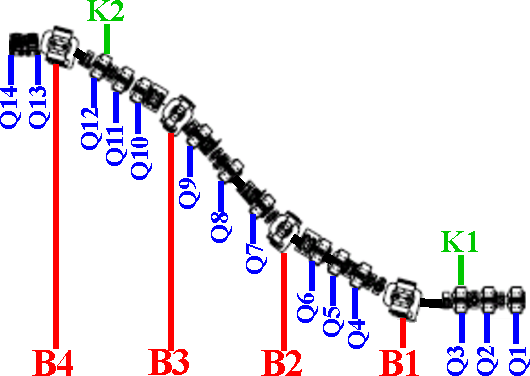
\includegraphics[width=0.5\columnwidth]{TL2Lattice_chicaneOnly}% 
  %Here is 
  %how to 
  %import EPS art
  \caption{\label{f:TL2Lattice}
  }
\end{figure}

The pre-existing TL2 chicane was already densely packed with magnets, and to 
maintain the functionality of the lattice for routine operation at CTF3 
elements could not be removed.
Space for the two PFF kickers (K1 and K2) was made available by rearranging 
quadrupoles in the line, moving quadrupoles with a wide aperture (Q3 and Q12) 
prior to the first (B1) and last (B4) dipole in the chicane.
The kickers are installed inside the aperture of these quadrupoles 
(Fig.~\ref{f:kickerInsideQuad}). 

\begin{figure}
  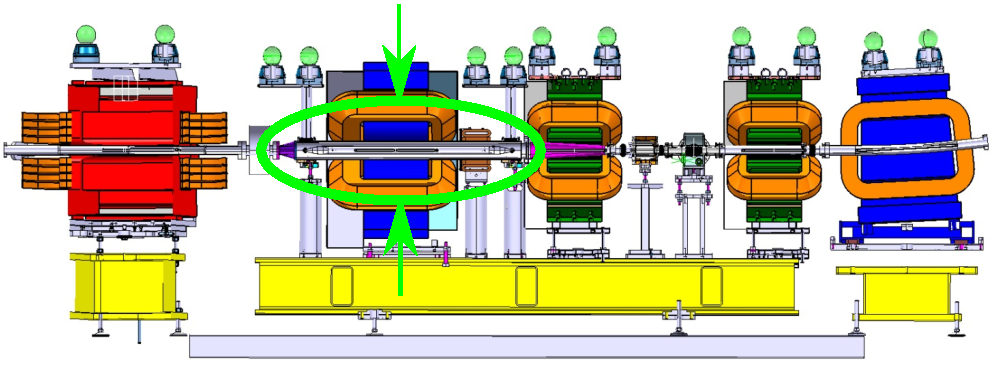
\includegraphics[width=\columnwidth]{kickerInsideQuad}% Here is 
  %how to 
  %import EPS art
  \caption{\label{f:kickerInsideQuad}
  }
\end{figure}

New optics for the TL2 line, maintaining the previous matching constraints 
required for normal operation and adding the new PFF constraints, were created 
using the CTF3 MADX model. The accuracy of the model for the rearranged line 
was verified and improved in a series of kick-response measurements [REF]. 
Relying on the pre-existing chicane layout forced several compromises in the 
chicane optics.

The original optics constraints include - matching combiner ring extraction and 
CLEX injection, dispersion closure and minimised, beta functions small/smooth. 
The additional PFF constraints ensure the phase (path length) dependence on the 
kicker voltages, and that the beam orbit downstream of the chicane is closed.

The rms beam energy spread at CTF3 is at the 1\% level. The beam pipe in the 
correction chicane has a diameter of 10~cm to give a large acceptance for the 
dispersion component of the beam size. However, the aperture of the PFF kickers 
is only 2~cm. The dispersion must be closed at the chicane exit and minimised 
at \(K_2\) (\(K_1\) is prior to the chicane in a dispersion free region). 

The correction range of the PFF system, or the dependence of the beam phase on 
the angular deflection applied at \(K_1\), is defined by the transfer matrix 
coefficient \(R_{52}\) between the two kickers:
\begin{equation}
\phi_{\mathrm{K2}} = \phi_i + R_{52}x'_{\mathrm{K1}}
\end{equation}
Maximising \(R_{52}\) has the 
unfortunate consequence of increasing the dispersion, thus the optics must be a 
compromise that achieves a reasonable
correction range whilst keeping the dispersion small enough to avoid beam 
losses.

The dispersion and phase shift for a 1~mrad kick at \(K_1\) in the matched 
optics for the chicane are shown in Fig.[REF] and Fig.[REF] respectively. An 
\(R_52\) value of 0.74~m 
is achieved (corresponding to a phase shift of \(-10.6^\circ\) per mrad at 
\(K_1\)) with 
a dispersion of [val] at \(K_2\). With this dispersion approximately [val] 
sigma of the beam energy distribution fits within the \(K_2\) aperture.

\begin{figure*}
 \centering
 \hfill
  \subfloat[][Horizontal and vertical beta function.]
  {
    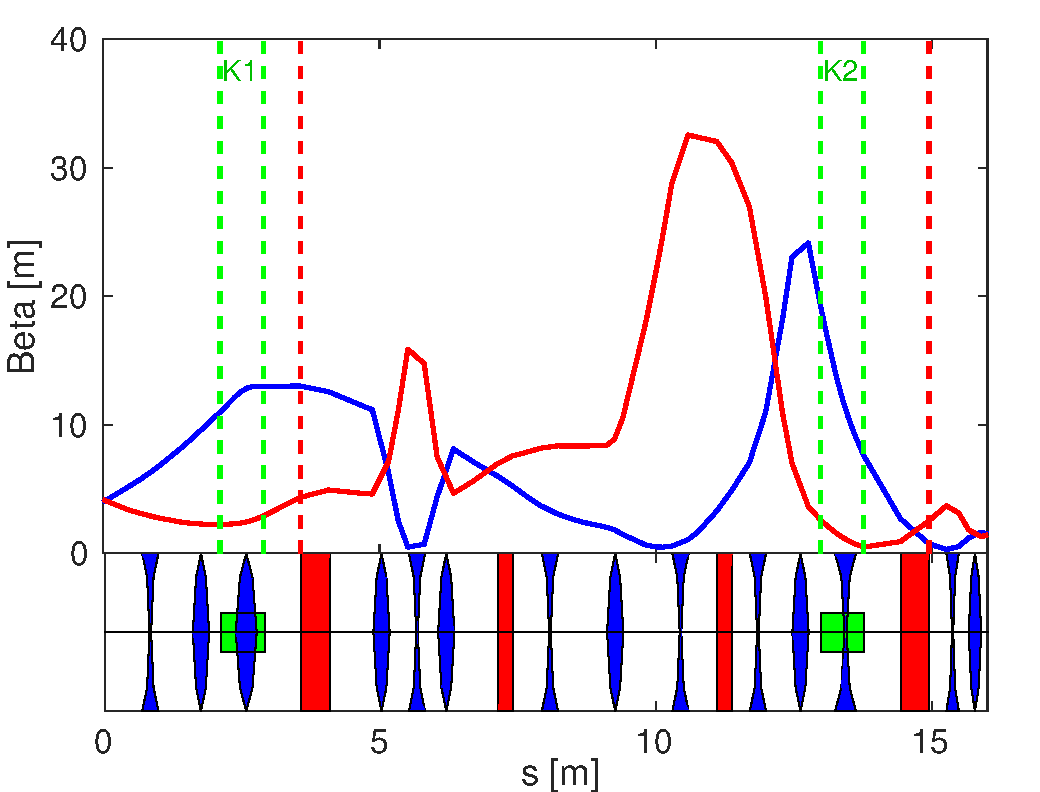
\includegraphics[width=0.49\textwidth]{pffOpticsBeta_chicane}
    \label{f:pffOpticsBeta}
  }
  \subfloat[][Horizontal dispersion.]
   {
    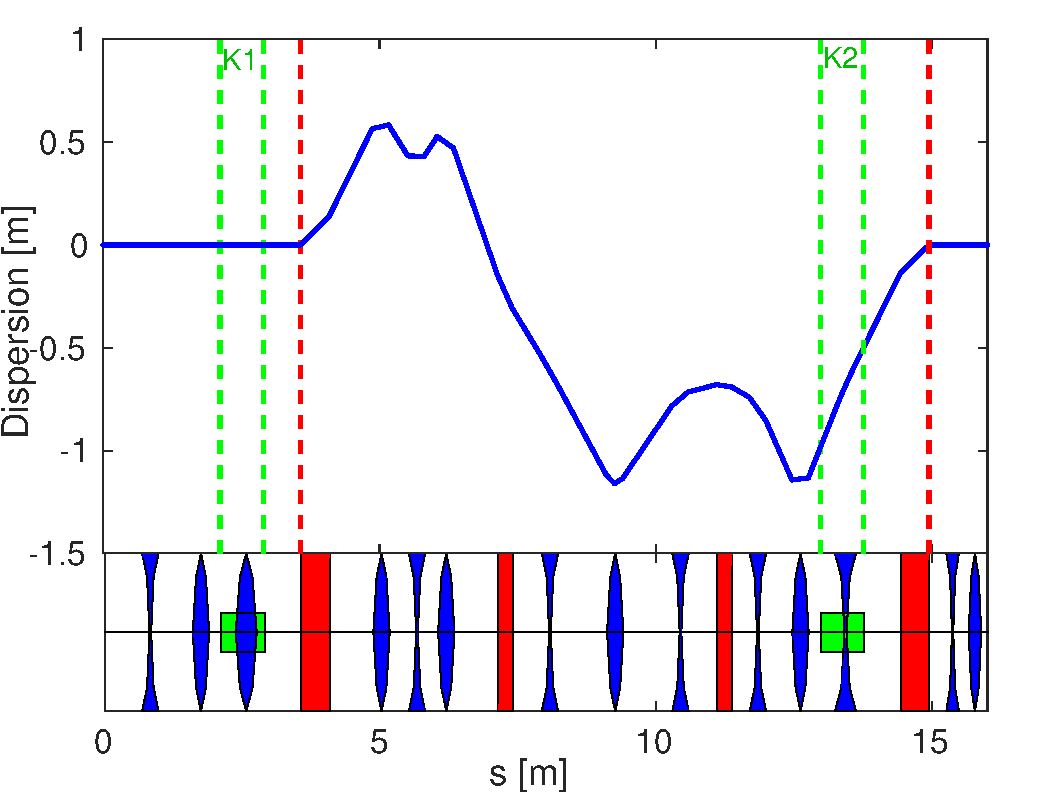
\includegraphics[width=0.49\textwidth]{pffOpticsDisp_chicane}
    \label{f:pffOpticsDisp_chicane}
    }

  \subfloat[][Phase shift for an applied kick of +1~mrad at K1 and -1~mrad at K2.]
   {
    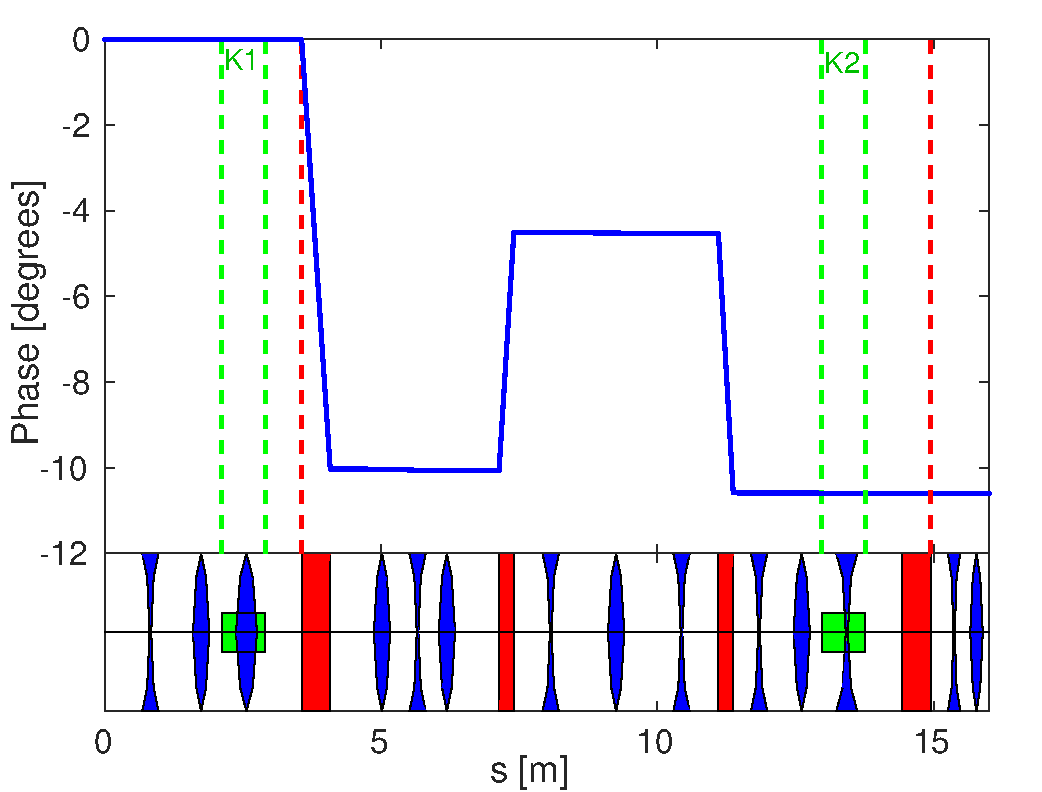
\includegraphics[width=0.49\textwidth]{pffOpticsPhase_chicane}
    \label{f:pffOpticsPhase_chicane}
    }
  \subfloat[][Horizontal orbit with an applied kick of  +1~mrad at K1 and -1~mrad at K2.]
   {
    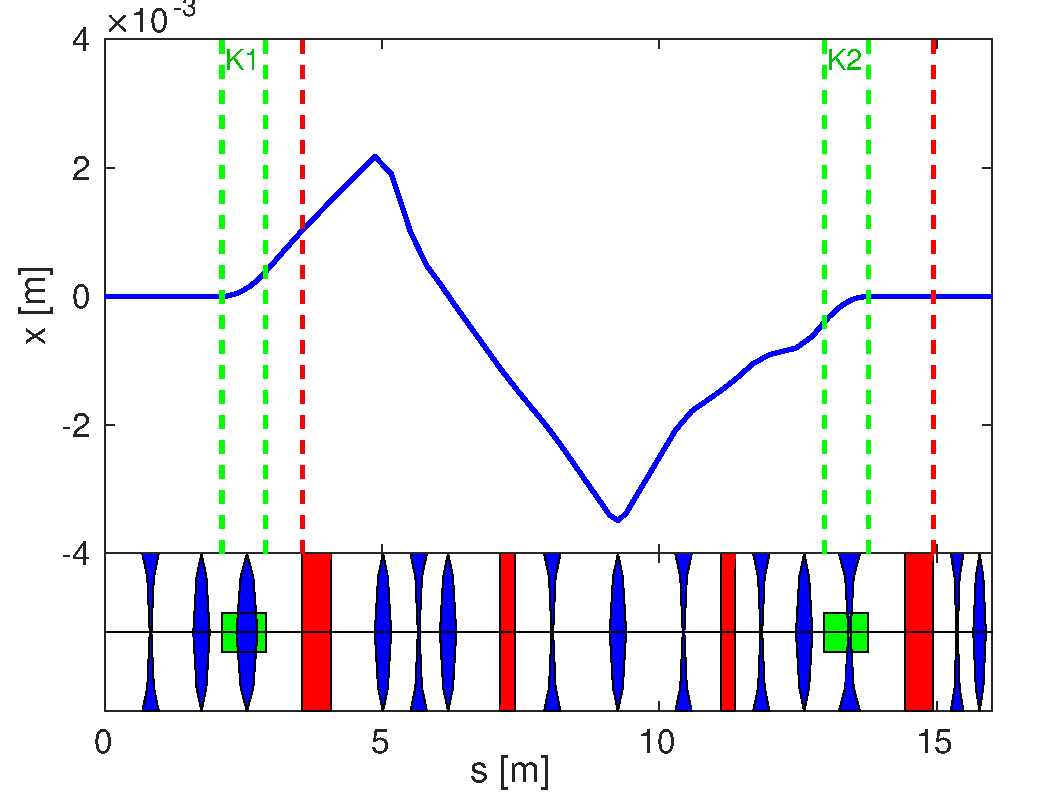
\includegraphics[width=0.49\textwidth]{pffOpticsX_chicane}
    \label{f:pffOpticsX_chicane}
   }

  \subfloat[][\(R_{56}\) coefficient.]
   {
    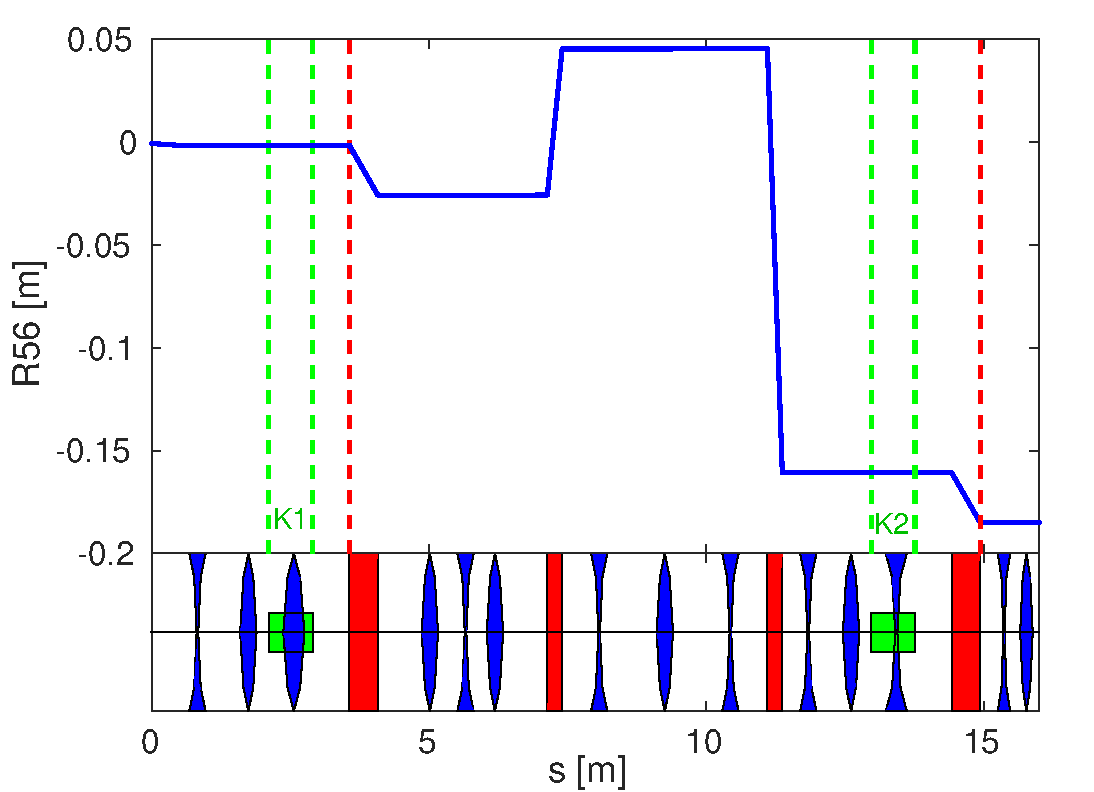
\includegraphics[width=0.49\textwidth]{pffOpticsR56_chicane}
    
    \label{f:pffOpticsR56_chicane}
    }

  \caption{\label{f:opticsPlots}Optics for the correction chicane. The 
  positions of quadrupoles (blue concave or convex lenses), dipoles (red 
  rectangles) and the PFF kickers (green squares) are indicated under each 
  plot.}

\end{figure*}

The last two figures, \ref{f:pffOpticsX}~and~\ref{f:pffOpticsPhase}, show the 
effect of kicking the beam with the PFF kickers. A deflection of +1~mrad is 
applied from the first kicker, and -1~mrad from the second kicker. This leads 
to a peak horizontal orbit offset of 3.5~mm inside the horizontal chicane. The 
orbit is closed at the \(10^{-7}\) level following the chicane, so that the 
beam's trajectory following the PFF system is independent of the applied kick. 

Finally, the \(R_{52}\) value between the two kickers is 0.74~m. This defines 
the phase shift resulting from kicking the beam in the chicane, which is the 
key figure of merit for the PFF system. As shown in 
Figure~\ref{f:pffOpticsPhase} a kick of 1~mrad provides a phase shift of 
\(-10.6^\circ\) in this optics. This is converted in to the actual range of the 
PFF system taking in to account the specifications of the kicker amplifiers in 
Chapter~\ref{c:commissioning}. Verifications of the performance of the optics 
are presented in Chapters~\ref{c:phasePropagation}~and~\ref{c:commissioning}.
% /FROM THESIS

\subsection{\label{ss:prop}Phase Propagation}

As in Eq.[ref] the corrected downstream phase jitter that the PFF system can 
achieve depends on the correlation between the upstream (input) phase and the 
initial downstream phase. This correlation is determined by the phase monitor 
resolution and any additional beam phase jitter introduced in-between 
\(\phi_u\) and \(\phi_d\). In the first measurements with the new correction 
chicane optics (such as Fig.\ref{f:origUpVsDown}) the correlation was below 
40\% and the downstream phase jitter more than two times larger than upstream. 

\begin{figure}
  \centering
  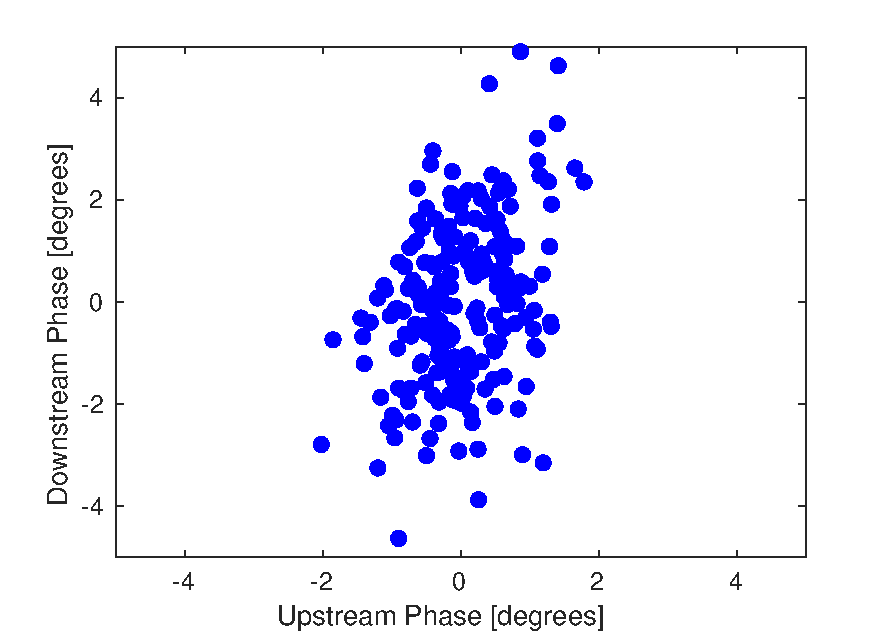
\includegraphics[width=0.6\columnwidth]{origUpVsDown}% Here is 
  %how to 
  %import EPS art
  \caption{\label{f:origUpVsDown} Upstream vs. downstream phase
  }
\end{figure}

% FROM THESIS
One constraint that could not be met in conjunction with the other chicane 
optics requirements was for the transfer matrix element \(R_{56}\) to be zero. 
\(R_{56}\) describes the dependence of the phase on the beam energy, to first 
order, as 
follows: 
\begin{equation}
\phi_d = \phi_u + R_{56}\frac{\Delta p}{p}
\label{e:r56PhasEq}
\end{equation}
Where \(R_{56}\) is the \(R_{56}\) coefficient between the upstream and 
downstream monitors, and \(\Delta p/p\) is the fractional energy offset.

As seen in Figure~\ref{f:pffOpticsR56} the \(R_{56}\) transfer matrix 
coefficient across the horizontal chicane is -0.18~m. As other beam lines at 
CTF3 nominally have \(R_{56}=0\), the total \(R_{56}\) between \(\phi_u\) and 
\(\phi_d\) is also -0.18~m. This leads to additional energy dependent phase 
jitter in \(\phi_d\) that is not present in \(\phi_u\).

\begin{figure}
  \centering
  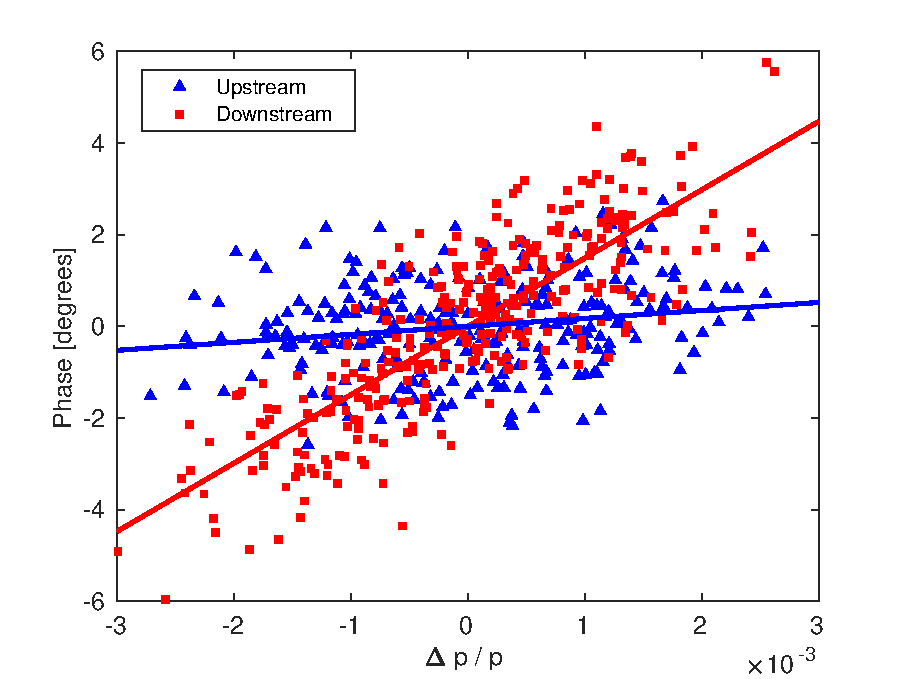
\includegraphics[width=0.6\columnwidth]{UpDownEnCorr}
  \caption{\label{f:UpDownEnCorr}
  }
\end{figure}

The effect of this is shown in Fig.~\ref{f:UpDownEnCorr}, in which the phase is 
plotted versus the beam energy (calculated using the beam position in a 
dispersive BPM). A correlation of [val] between the upstream phase and the beam 
energy is amplified to [val] downstream.

From Equations [val] and [val] the effect of \(R_{56}\) on the correlation and 
the PFF performance can be derived [REF]. Excluding the phase monitor 
resolution, the 
corrected downstream phase jitter that can be achieved is given by:
% FROM THESIS
%\begin{equation}
%\rho_{ud} = \frac{\sigma_u + R_{56}\rho_{up}\sigma_p}{\sqrt{\sigma_u^2 + 
%    R_{56}^2\sigma_{p}^2 + 2R_{56}\rho_{up}\sigma_{u}\sigma_{p}}}
%\label{e:r56CorrDefFinal}
%\end{equation}
\begin{equation}
\sigma_{PFF} = \left|R_{56}\right|\sigma_p\sqrt{1-\rho_{up}^2}
\label{e:r56PFFJit}
\end{equation}
Where \(\sigma_p\) is the beam energy jitter (typically [val] at CTF3) and 
\(\rho_{up}\) is the correlation between the upstream phase and the beam energy 
(typically [val]). Fig.\ref{f:jitVsR56} shows the dependence of the initial and 
corrected downstream phase jitter on the \(R_{56}\) value. The slight asymmetry 
between positive and negative \(R_{56}\) values is caused by the non-zero 
correlation between the upstream phase and the beam energy. To reduce a typical 
initial beam jitter of \(0.8^\circ\) at CTF3 to the CLIC target of 
\(0.2^\circ\), the \(R_{56}\) value between the upstream and downstream 
monitors must be less than [val].

%\begin{figure}
%  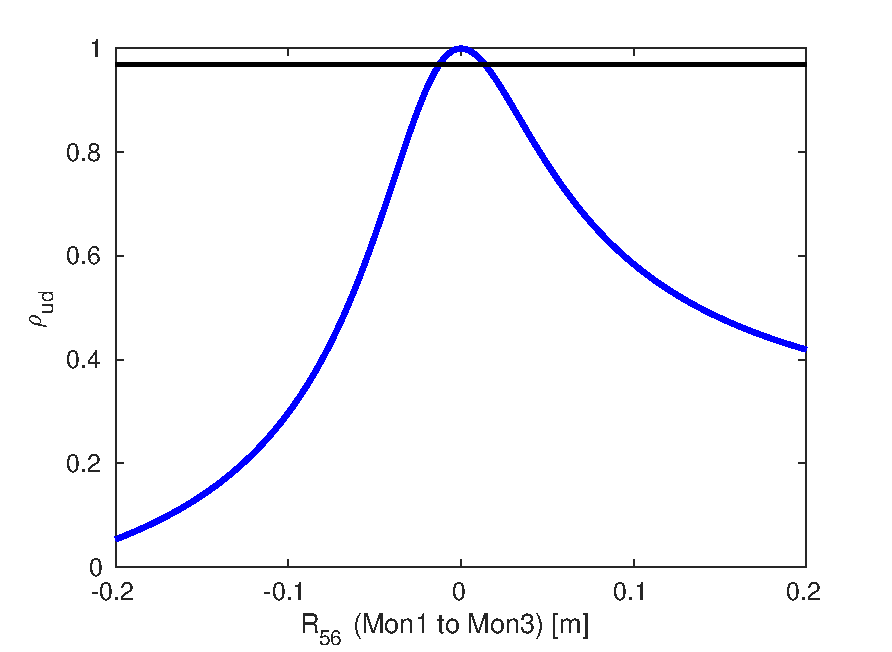
\includegraphics[width=\columnwidth]{corrVsR56}
%  \caption{\label{f:corrVsR56}
%  }
%\end{figure}
\begin{figure}
 \centering
  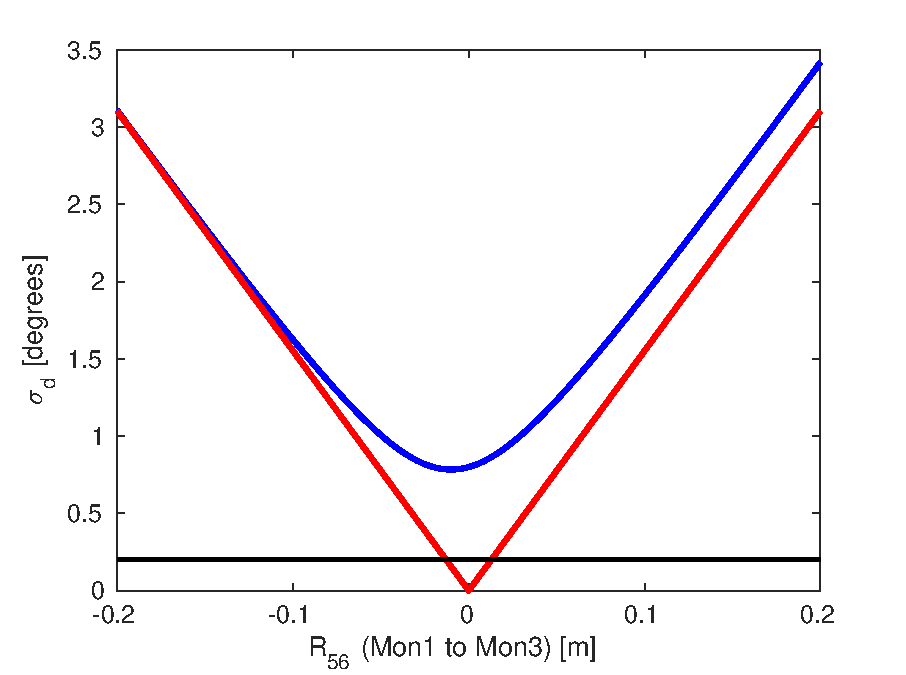
\includegraphics[width=0.6\columnwidth]{jitVsR56}
  \caption{\label{f:jitVsR56}
  }
\end{figure}


To compensate, messed around with TL1... R56 scan...

Optimal \(R_{56}\) value not constant... correlation variations along pulse... 
hinted at higher order effects... Second order phase-energy dependence in the 
optics is described using the \(T_{566}\) matrix coefficient:
\begin{equation}
\phi_d = \phi_u + R_{56}\left(\frac{\Delta p}{p}\right) + 
T_{566}\left(\frac{\Delta p}{p}\right)^2
\label{e:t566}
\end{equation}

%\begin{equation}
%R_{56} = -2T_{566} \left(\frac{\Delta p}{p}\right)
%\label{e:r56t566dep}
%%\end{equation}
%/FROM THESIS

% FROM THESIS
Fig.~\ref{f:R56ScanGunWiggle_PhaseVsEnergy} shows the dependence of the mean 
downstream phase on the beam energy for three different \(R_{56}\) values set 
in TL1: \(-0.1\)~m, \(0.075\)~m and \(0.3\)~m. The beam energy was varied 
during the data taking period, and the second order term becomes clear.
% /FROM THESIS


%\begin{figure}
%  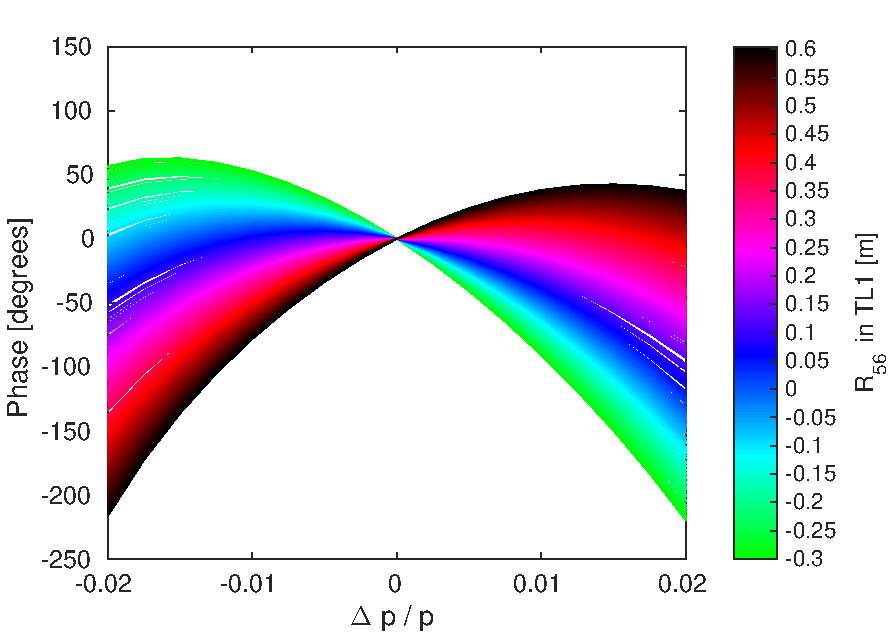
\includegraphics[width=\columnwidth]{phaseVsEn_t566}% Here is 
%  %how to 
%  %import EPS art
%  \caption{\label{f:phaseVsEn_t566}
%  }
%\end{figure}

\begin{figure}
 \centering
  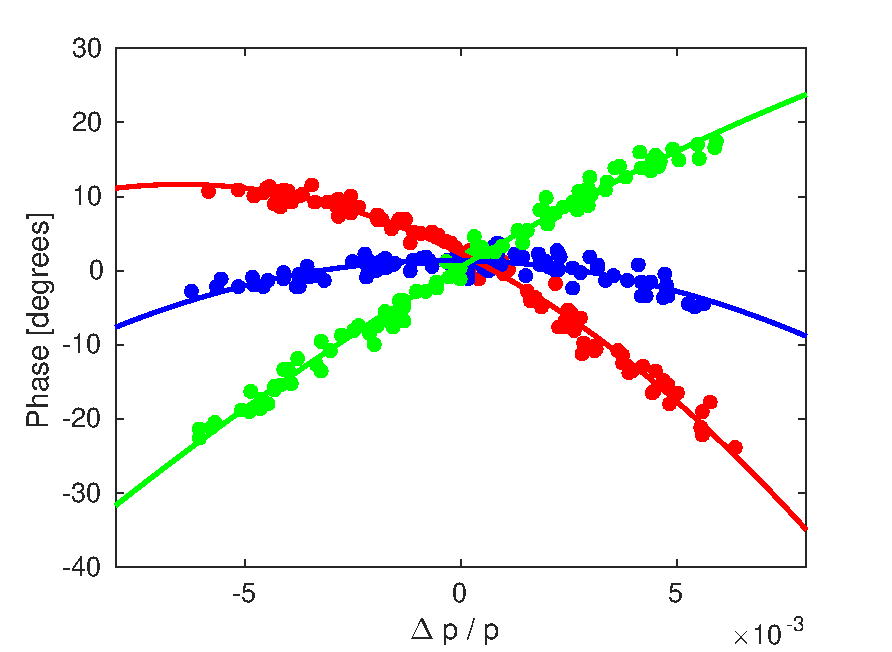
\includegraphics[width=0.6\columnwidth]{R56ScanGunWiggle_PhaseVsEnergy}%
  % Here is 
  %how to 
  %import EPS art
  \caption{\label{f:R56ScanGunWiggle_PhaseVsEnergy}
  }
\end{figure}

Figs.~\ref{f:corrVsEnergyOffset}~and~\ref{f:maxCorrWithT566} shows the effect 
of \(T_{566}\) on the correlation for different beam energy offsets and beam 
energy jitters respectively. In each case it is assumed the first order 
\(R_{56}\) has been completely cancelled using TL1. energy jitter/offset [val] 
assumed.

\begin{figure*}
 \hfill
  \subfloat
   {
    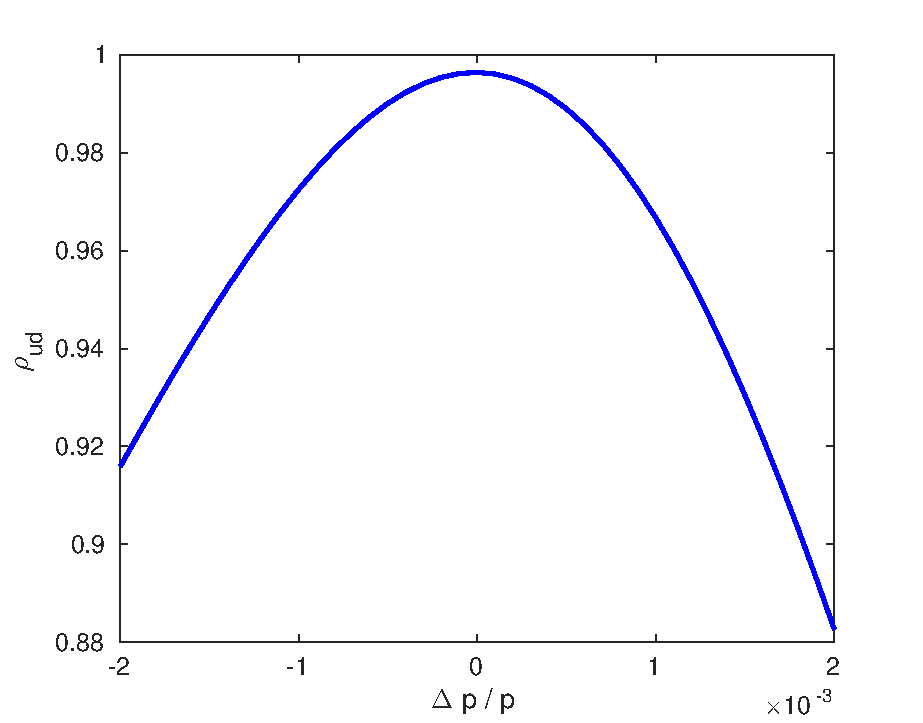
\includegraphics[width=0.5\textwidth]{corrVsEnergyOffset}
    \label{f:corrVsEnergyOffset}
    }
  \subfloat
   {
    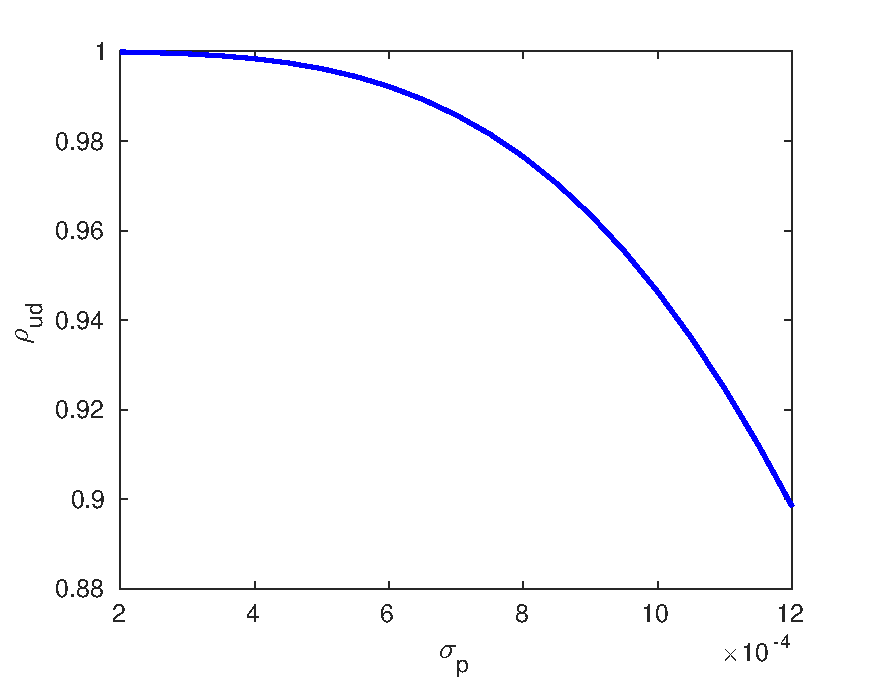
\includegraphics[width=0.5\textwidth]{maxCorrWithT566}
    \label{f:maxCorrWithT566}
   }
\end{figure*}

In optimal conditions CTF3 energy jitter as low as [val] and variations along 
pulse below [val], which means not a limiting factor to achieve 0.2 degrees. 
But the sensitivity to energy drifts made it difficult/impossible to maintain 
peak PFF performance on long time scales. CLIC application would require 
\(R_{56}\) and \(T_{566}\) to be zero in the turnarounds.

